\documentclass{article}
\usepackage{tikz}
\begin{document}
    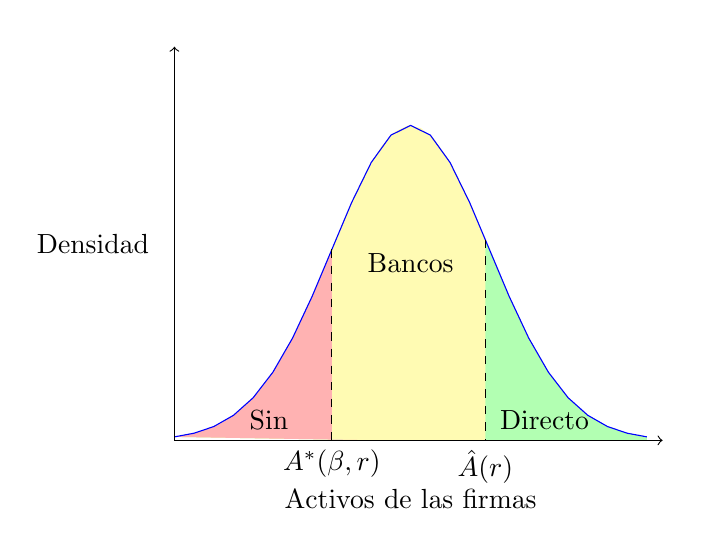
\begin{tikzpicture}
    % define normal distribution function 'normaltwo'
    \def\normaltwo{\x,{4*1/exp(((\x-3)^2)/2)}}
    
    % input y parameter
    \def\y{2.0}
    \def\z{3.95}
    \def\w{6.0}
    % this line calculates f(y)
    \def\fy{4*1/exp(((\y-3)^2)/2)}
    \def\fz{4*1/exp(((\z-3)^2)/2)}
    \def\fw{4*1/exp(((\w-3)^2)/2)}
    
    % Shade orange area underneath curve.
   \fill [fill=green!30] (2.6,0) -- plot[domain=0:6.0] (\normaltwo) -- ({\w},0) -- cycle;
    
    \fill [fill=yellow!30] (2.6,0) -- plot[domain=0:3.95] (\normaltwo) -- ({\z},0) -- cycle;
    
     \fill [fill=red!30] (2.6,0) -- plot[domain=0:2.0] (\normaltwo) -- ({\y},0) -- cycle;
    % Draw and label normal distribution function
    \draw[color=blue,domain=0:6] plot (\normaltwo) node[right] {};
    
    % Add dashed line dropping down from normal.
    \draw[dashed] ({\y},{\fy}) -- ({\y},0) node[below] {$A^{*}(\beta, r)$};
    \draw[dashed] ({\z},{\fz}) -- ({\z},0) node[below] {$\hat{A}(r)$};
    
    % Optional: Add axis labels
    \draw (-.2,2.5) node[left] {Densidad};
    \draw (3,-.5) node[below] {Activos de las firmas};
    
    % Optional: Add axes
    \draw[->] (0,0) -- (6.2,0) node[right] {};
    \draw[->] (0,0) -- (0,5) node[above] {};
    
    \node[below] at (1.2,0.5) {Sin};
    \node[below] at (3.0,2.5) {Bancos};
    \node[below] at (4.7,0.5) {Directo};
    \end{tikzpicture}
\end{document}